\chapter{LSPE/Strip}

\section{The LSPE Experiment}

\begin{figure}
        \centering
        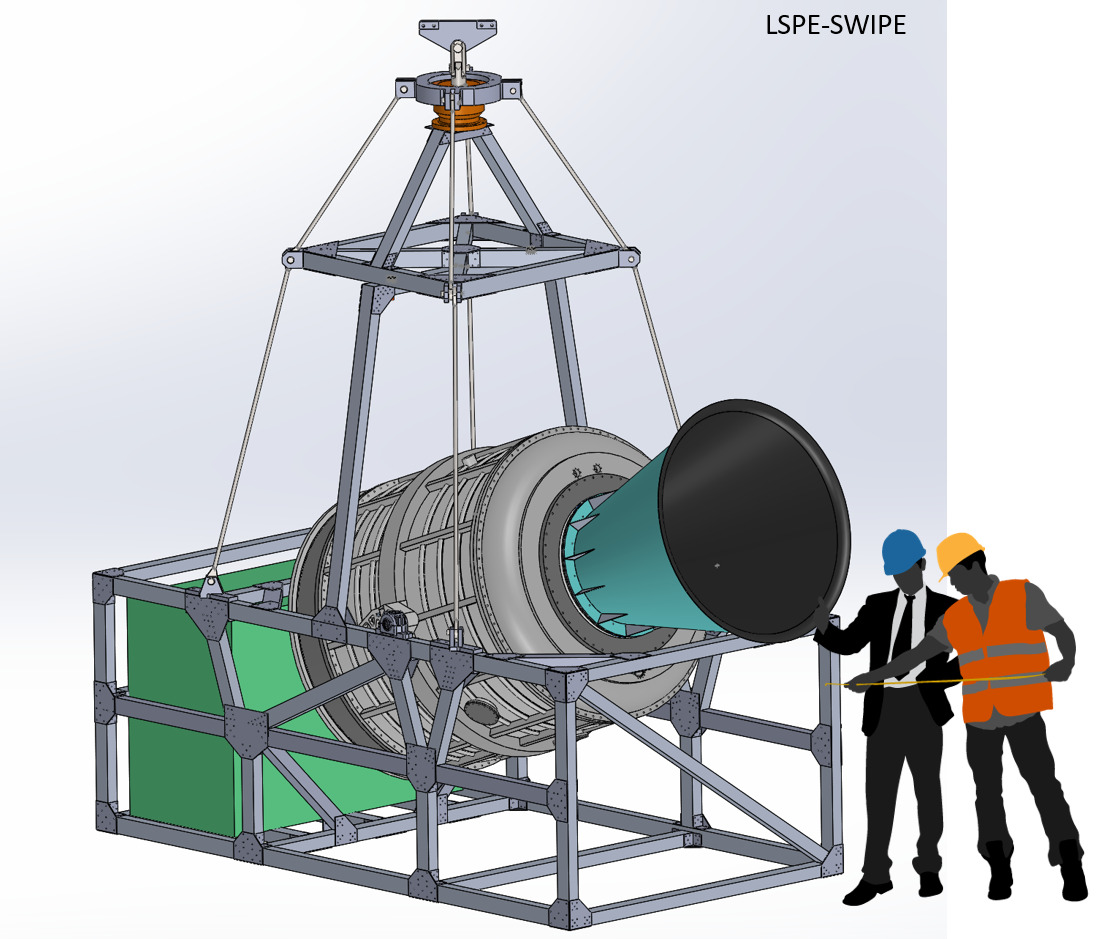
\includegraphics[width=\textwidth]{SWIPE}
        \caption{The SWIPE instrument}
        \label{fig:swipe}
\end{figure}

\section{The Strip Instrument}

\begin{figure}
        \centering
        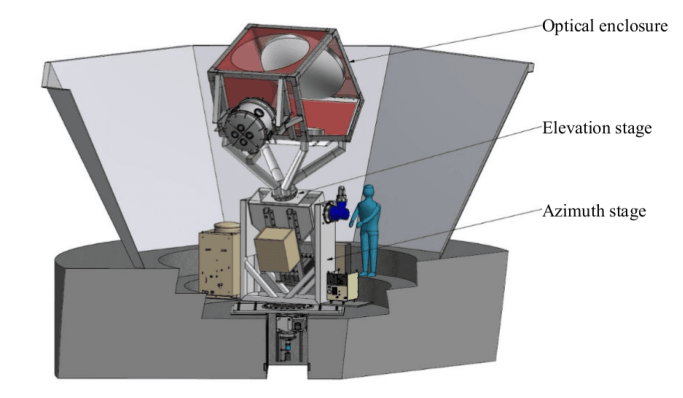
\includegraphics[width=\textwidth]{LSPE-Strip-optical-system}
        \caption{LSPE/Strip Optical System}
        \label{fig:lspe-strip_optical_system}
\end{figure}

\begin{figure}
        \centering
        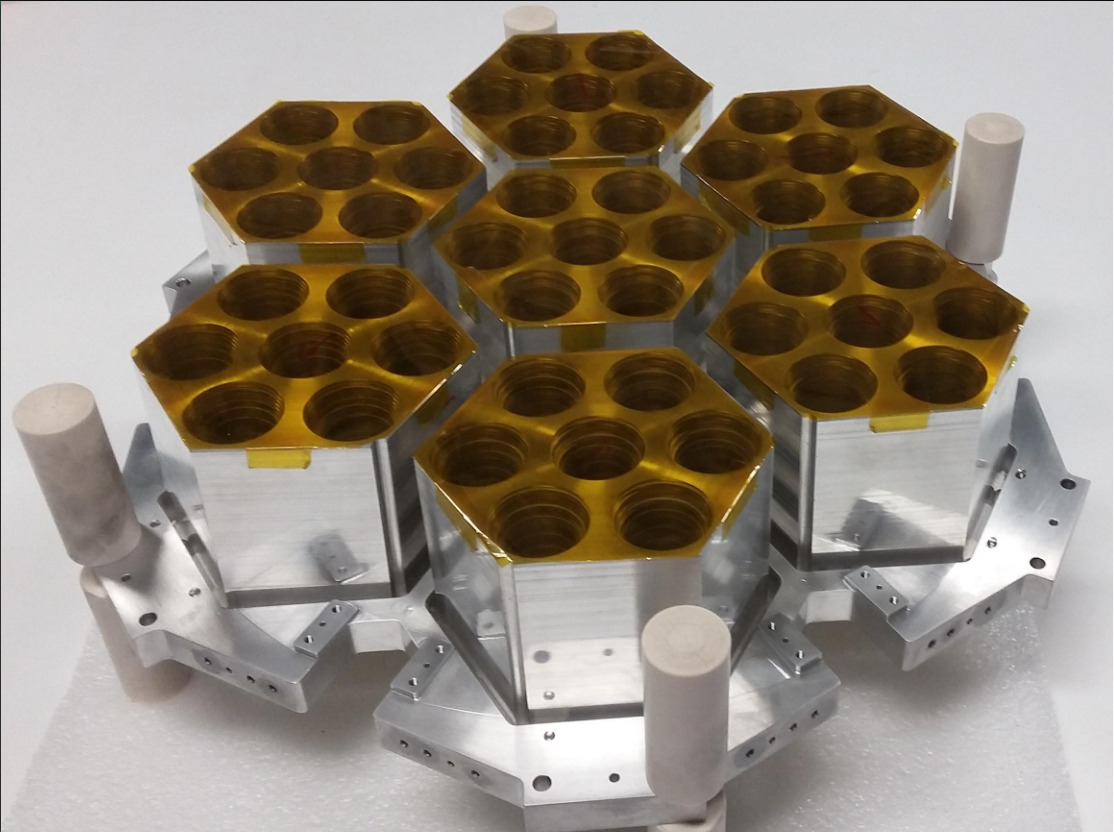
\includegraphics[width=\textwidth]{strip-focal-plane}
        \caption{Strip focal plane}
        \label{fig:strip_focal_plane}
\end{figure}

\subsection{The Observation Site}

The Strip instrument will be deployed to the \emph{Observatorio del Teide}
in the city of Iza\~na, in Tenerife Island, Spain (\ang{28;18;04} N,
\ang{16;30;38} W) (see \autoref{fig:observatorio_teide}). The astronomical
observatory is located on Mount Teide at \SI{2390}{\meter} above sea level
and it has been operated by the \emph{Instituto de Astrof\'isica de
Canarias} since 1964.

The Observatory's geographical location, combined with the excellent
quality of the sky for astronomy, led to Teide Observatory being dedicated
mainly to  the study of the sun. However, Teide Observatory hosted and
still hosts different CMB experiments.
The \emph{Tenerife Experiment} (1984) by Jodrell Bank (of the University of
manchester) was the first CMB experiment to be installed at the
observatory. It measured CMB temperature anisotropies on angular size of
\ang{5}. Currently the observatory hosts the \emph{Multi Frequency
Instrument} (MFI), the \emph{Thirty Gigahertz Instrument} (TGI) and the
\emph{Forty Gigahertz Instrument} (FGI) of the \emph{Q-U-I JOint TEnerife
CMB} (QUIJOTE-CMB) experiment by the Instituto de Astrof\'isica de
Canarias. QUIJOTE experiment aims to characterize the
polarization of the CMB radiation in the frequency range
\SIrange{10}{42}{\giga\hertz}. The Strip instrument will join the
international efforts to detect the B-modes of the CMB polarization,
observing the microwave sky from the same site.

The characteristic geographical and climatic non-homogeneity typical of
relatively small islands constitutes a challenge for the estimate of the
systematics linked to atmospheric effects. This problem will be tackled in
the next chapters of this thesis.



\begin{figure}
        \centering
        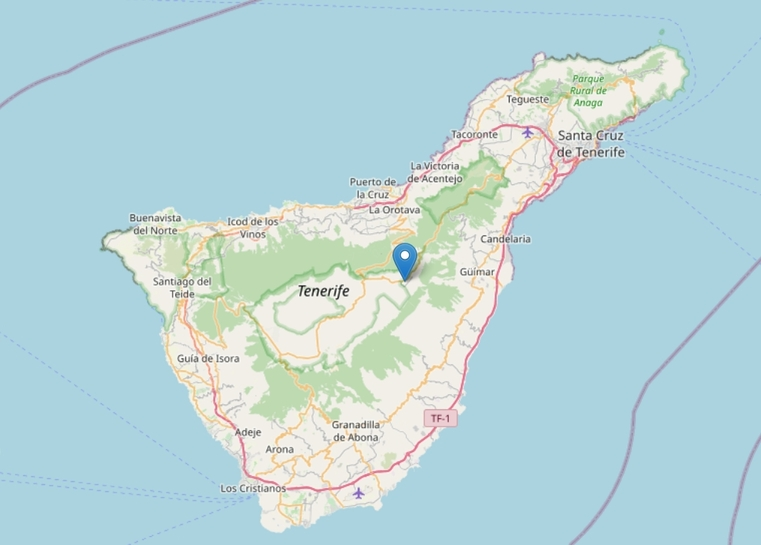
\includegraphics[width=\textwidth]{observatorio_teide}
        \caption{Observatorio del Teide}
        \label{fig:observatorio_teide}
\end{figure}

